\documentclass[conference]{IEEEtran}

\usepackage{newtxtext,newtxmath}
\usepackage{amsmath}
\usepackage{booktabs}
\usepackage{graphicx}
\usepackage{longtable}
\usepackage{array}
\usepackage{url}
\usepackage[hidelinks]{hyperref}
\usepackage{tikz}
\usetikzlibrary{arrows.meta}

\urlstyle{tt}
\setlength{\emergencystretch}{3em}
\newcolumntype{L}[1]{>{\raggedright\arraybackslash}p{#1}}
\newcommand{\codepath}[1]{{\Urlmuskip=0mu plus 1mu\relax\nolinkurl{#1}}}

\begin{document}

\title{DC Energy Optimization}

\author{\IEEEauthorblockN{Janusz Gal}
\IEEEauthorblockA{jgal@charlotte.edu}}

\maketitle

\begin{abstract}
TODO: abstract.
\end{abstract}

\begin{IEEEkeywords}
data centers, demand response, grid ramp, reinforcement learning, workload
scheduling
\end{IEEEkeywords}

\section{Google ClusterData2019 Workload Trace}
\label{sec:clusterdata2019}

\subsection{Dataset}
\label{subsec:clusterdata-role}

A \emph{Borg cell} is a cluster of thousands of machines in a Google Data Center, which recieve and process IT actions known as jobs. Google provides a detailed record of 8 such cells, labeled \(a\)--\(h\), from a May 2019 data capture \cite{wilkes2020clusterdata2019}. Each cell record contains machine capacity, per-instance resource usage, job submission events, priorities, and resource requests. Each record is also sanitized, meaning no user,application, geography, or other identifiable information is given. 

The full dataset is 2.4 TiB, so we use \emph{BigQuery} to query the data and export relevant tables to be consumed downstream. Three \emph{BigQuery} tables produce the data this experiment consumes --- \codepath{machine_events} for capacity, \codepath{instance_usage} for measured CPU, and \codepath{collection_events} for priority. Table~\ref{tab:clusterdata-upstream-fields} in Appendix~\ref{app:source-tables} gives the exact fields within each table that we consume.

\begin{figure}[!ht]
  \centering
  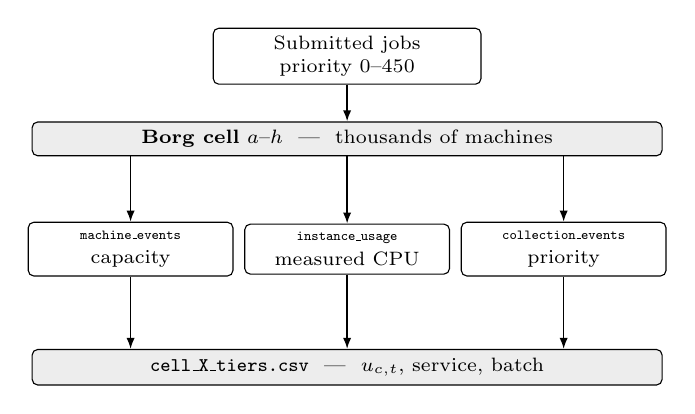
\begin{tikzpicture}[
    font=\scriptsize,
    box/.style={draw, rounded corners=2pt, align=center, inner sep=3pt},
    shaded/.style={box, fill=black!7},
    arr/.style={-{Latex[length=1.4mm]}, semithick}
  ]
    \node[box, minimum width=34mm] (jobs) at (0,0)
      {Submitted jobs\\priority 0--450};

    \node[shaded, minimum width=80mm] (cell) at (0,-1.05)
      {\textbf{Borg cell} \(a\)--\(h\)\ \ ---\ \ thousands of machines};

    \node[box, minimum width=26mm] (me) at (-2.75,-2.45)
      {\texttt{\tiny machine\_events}\\[1pt]capacity};
    \node[box, minimum width=26mm] (iu) at (0,-2.45)
      {\texttt{\tiny instance\_usage}\\[1pt]measured CPU};
    \node[box, minimum width=26mm] (ce) at (2.75,-2.45)
      {\texttt{\tiny collection\_events}\\[1pt]priority};

    \node[shaded, minimum width=80mm] (csv) at (0,-3.95)
      {\texttt{cell\_X\_tiers.csv}\ \ ---\ \ \(u_{c,t}\), service, batch};

    \draw[arr] (jobs) -- (cell);
    \draw[arr] (cell.south -| me) -- (me.north);
    \draw[arr] (cell.south -| iu) -- (iu.north);
    \draw[arr] (cell.south -| ce) -- (ce.north);
    \draw[arr] (me.south) -- (me.south |- csv.north);
    \draw[arr] (iu.south) -- (iu.south |- csv.north);
    \draw[arr] (ce.south) -- (ce.south |- csv.north);
  \end{tikzpicture}
  \caption{Extraction path from the Google trace to the retained tier curves.}
  \label{fig:clusterdata-pipeline}
\end{figure}


\subsection{Compute utilization extraction}
\label{subsec:clusterdata-utilization}

Within the \emph{ClusterData2019} dataset, Google normalizes CPUs so that the largest machine capacity is simply 1.0 unit. Our goal with this data is to provide a fraction of each cell's CPUs that were busy. This ratio is defined as:

\begin{equation}
  u_{c,t}
  =
  \frac{\sum_{i\in\mathcal{U}_{c,t}} a_i}
       {\sum_{j\in\mathcal{M}_c} \kappa_j},
  \label{eq:clusterdata-utilization}
\end{equation}
where \(\mathcal{U}_{c,t}\) is the set of \codepath{instance_usage} records for cell \(c\)
in five-minute bucket \(t\) that survive the two filters below, \(a_i\) is the
\codepath{average_usage.cpus} rate of record \(i\), \(\mathcal{M}_c\) is the set
of machines in cell \(c\), and \(\kappa_j\) is the largest
\codepath{capacity.cpus} ever reported for machine \(j\).\footnote{A machine can appear several times in \codepath{machine_events}, through add, update, and snapshot records, so we take each machine's largest reported capacity and sum across machines. This picks the largest \emph{capacity} record, not the busiest moment.} Both sums are in Google's normalized CPU units, so \(u_{c,t}\) is dimensionless and saved as the \codepath{cpu_demand_norm} column.

The two filters for the instance-usage records are:

\begin{itemize}
  \item \textbf{Top-level instances only.} Google's trace lets a task run         inside an \emph{allocation set}, a reserved block of resources that is         itself a task. Counting both the allocation set and the tasks inside it         would count the same CPU twice, so we keep only records whose \codepath{alloc_collection_id} is null or zero (\codepath{NO_ALLOC_COLLECTION}) \cite{googleTraceFormatV3}. Google's analysis notebook calls these ``top-level instances.''
  \item \textbf{Complete windows only.} A usage record that covers less than the full five minutes is dropped. The trace emits a partial record when an instance starts or stops mid-window. Adding it in as though it covered all five minutes would overstate that instance. Requiring at least 300 seconds gives every retained row the same duration. 
\end{itemize}

The final output is one file per cell, \codepath{data/cells/cell_X_tiers.csv}, with columns \codepath{timestep}, \codepath{cpu_demand_norm}, \codepath{batch_share}, \codepath{service_demand_norm}, and \codepath{batch_demand_norm}.

\begin{table*}[t]
  \centering
  \small
  \caption{The five columns of \codepath{data/cells/cell_X_tiers.csv}, with real values from cell \(a\) at three buckets: its quietest, its median, and its busiest. Every utilization column is a dimensionless fraction of the cell's total CPU capacity, so the three of them are directly comparable.}
  \label{tab:clusterdata-tier-columns}
  \begin{tabular}{@{}L{0.24\textwidth}L{0.36\textwidth}rrr@{}}
    \toprule
     & & \multicolumn{3}{c}{Cell \(a\)} \\
    \cmidrule(l){3-5}
    Column & What it holds & Quiet & Median & Busy \\
    \midrule
    \codepath{timestep}
      & Index of the five-minute bucket, counting from the start of the trace;
        0 to 8{,}928 covers all of May 2019.
      & 255 & 5257 & 2681 \\
    \addlinespace
    \codepath{cpu_demand_norm}
      & All measured CPU consumption in the bucket, divided by the cell's total
        CPU capacity.
      & 0.3320 & 0.5652 & 0.6931 \\
    \addlinespace
    \codepath{service_demand_norm}
      & The part of that consumption \emph{not} identified as deferrable:
        priority above 115, or no matched priority record at all.
      & 0.2432 & 0.4416 & 0.6341 \\
    \addlinespace
    \codepath{batch_demand_norm}
      & The part matched to a priority of 115 or below --- the free and
        best-effort tiers, which carry no service-level objective.
      & 0.0888 & 0.1236 & 0.0590 \\
    \addlinespace
    \codepath{batch_share}
      & \codepath{batch_demand_norm} divided by \codepath{cpu_demand_norm}.
        Derived for inspection; nothing downstream reads it.
      & 0.2675 & 0.2187 & 0.0851 \\
    \bottomrule
  \end{tabular}
\end{table*}


\subsection{Service and deferrable-batch split}
\label{subsec:clusterdata-tier-split}

The experiment relies on shifting compute demands (generated by jobs) to different locations and different times. To understand which demand can be shfited temporally, we rely on job priority defined by \codepath{collection_events}.  

Every submitted job carries a priority which Google groups into various bands. The two lowest bands (``free'' and ``best-effort batch,'' together everything at priority 115 or below) carry no service-level objective: the Borg cell may run this work whenever there is room, and may evict it when something more important needs the machine \cite{googleClusterAnalysisColab}. We refer to this as batch demand. All other priorities are seen as service demand and must be served on arrival.

Priority lives in \codepath{collection_events}, while usage lives in \codepath{instance_usage}, so the extraction builds one priority record per submitted job and joins it to usage by \codepath{collection_id}. Within each five-minute bucket, batch CPU is the usage matched to a priority at or below 115, normalized by the same cell capacity as before. Service CPU is aggregate minus batch, so the two components add back to the measured total at every timestep. The output of this extraction is two demand curves - the \codepath{service_demand_norm} and \codepath{batch_demand_norm}, for every 5 minute bucket.\footnote{Note it may be cleaner to refer to these as usage/consumption curves, but we are quantifying them as demand on the datacenter.}

\subsection{Reproducing the results}
\label{subsec:clusterdata-artifacts}

Re-running the extraction needs a Google Cloud project with BigQuery  enabled: \codepath{extract_tier_curves.ipynb} for cells \(a\)--\(d\), \codepath{extract_cells_eh.ipynb} for \(e\)--\(h\). What the repository keeps is the small tier CSVs, which are what everything downstream reads. 

\section{Google PowerData2019 Power Model}
\label{sec:powerdata2019}

\subsection{Datasets}
\label{subsec:powerdata-purpose}

The previous section essentially produced a \codepath{.csv} with details on how busy each cell was every 5 minutes. To convert this to energy that the datacenter demand required, we use \emph{PowerData2019}, also provided by Google as part of the Cluster Data. \emph{PowerData2019} provides 5 minute, per cell, normalized power utilization for the server equimpent. Since it is also normalized, we later state an assumption on the total power rating of a given datacenter.

We take the average of \codepath{measured_power_util} in a given hour, and pair this with average CPU utilization for the same hour. Each cell is then fitted with an orindary least squares line, allowing us to define a cell's power usage by it's normalized CPU utilization. This can be writen as:
\begin{equation}
  \widehat{p}_{c}(u)
  =
  \alpha_c + \beta_c u,
  \label{eq:powerdata-affine-fit}
\end{equation}

Where \(u\) is normalized CPU utilization and \(\widehat{p}_c\) is the predicted fraction of the cell's power capacity, \(\alpha_c\) is the idle draw and \(\beta_c\) is how much more it pulls when driven from idle to fully busy. 

\subsection{Fitted coefficients}
\label{subsec:powerdata-coefficients}

The coefficients are stored in \codepath{data/power_model_params.json}, fitted on 745 joined hourly observations per cell.

\begin{table}[htbp]
  \centering
  \footnotesize
  \caption{Per-cell CPU-only affine PowerData2019 fits.}
  \label{tab:powerdata-coefficients}
  \begin{tabular}{@{}crrrrr@{}}
    \toprule
    Cell & \(\alpha_c\) & \(\beta_c\) & \(\alpha_c+\beta_c\)
         & \(R^2\) & Joined hours \\
    \midrule
    \(a\) & 0.528016 & 0.339728 & 0.867743 & 0.7885 & 745 \\
    \(b\) & 0.548190 & 0.375761 & 0.923951 & 0.7479 & 745 \\
    \(c\) & 0.439604 & 0.525740 & 0.965344 & 0.7642 & 745 \\
    \(d\) & 0.382039 & 0.570370 & 0.952409 & 0.8005 & 745 \\
    \(e\) & 0.388045 & 0.601116 & 0.989161 & 0.9062 & 745 \\
    \(f\) & 0.427230 & 0.440739 & 0.867969 & 0.6472 & 745 \\
    \(g\) & 0.456218 & 0.492296 & 0.948515 & 0.7938 & 745 \\
    \(h\) & 0.383827 & 0.392821 & 0.776648 & 0.9432 & 745 \\
    \bottomrule
  \end{tabular}
\end{table}

\section{Energy Data}
\label{sec:energy-data}

Four markets are used for energy data: CAISO NP15 (northern California), MISO Minnesota, SPP North, and ISO-NE NEMA (greater Boston), all using the same EIA schema. This data is pulled from September 2025 to Februrary 2026. We intentionally use the most recent grid data to align with how demand shifting would impact todays grids, rather than 2019.\footnote{More than 31 days are required to allow the agent iteself to have seperate training and validation data.}

\subsection{Actual price and physical sources}
\label{subsec:energy-sources}

\begin{table*}[t]
  \centering
  \small
  \caption{Source products used in the active four-market panel.}
  \label{tab:energy-sources}
  \begin{tabular}{@{}L{0.14\textwidth}L{0.37\textwidth}L{0.41\textwidth}@{}}
  \toprule
  Market case & Day-ahead price & Physical demand and renewables \\
  \midrule
  CAISO NP15
    & CAISO OASIS \codepath{PRC_LMP} v12,
      \codepath{TH_NP15_GEN-APND}, total DAM LMP
      \cite{caisoOasis}
    & EIA CAISO balancing-authority demand, wind, and solar from
      \codepath{EBA.zip}. \\
  MISO Minnesota
    & Daily DA ex-post LMP report at \codepath{MINN.HUB}
      \cite{misoReports}
    & EIA MISO balancing-authority demand, wind, and solar. \\
  SPP North
    & SPP DA-LMP by settlement location at
      \codepath{SPPNORTH_HUB} \cite{sppPublicData}
    & EIA SPP balancing-authority demand, wind, and solar. \\
  ISO-NE NEMA
    & Final daily \codepath{WW_DALMP_ISO} report at NEMA/Boston location 4008
      \cite{isoneReports}
    & EIA ISO New England balancing-authority demand, wind, and solar. \\
  \bottomrule
  \end{tabular}
\end{table*}

Each source names its fields differently, so all four are rewritten into one common schema: EIA's \codepath{D}, \codepath{NG.WND}, and \codepath{NG.SUN} become \codepath{gross_demand_mw}, \codepath{wind_mw}, and \codepath{solar_mw}, and prices become \codepath{da_lmp_usd_per_mwh}. Table~\ref{tab:energy-example-rows} shows real rows at one shared hour, which is what the resultant files contain. 

\begin{table}[htbp]
  \centering
  \footnotesize
  \caption{Canonical four-market examples at 2025-10-10 00:00 UTC. Physical
  columns are MW; day-ahead LMP is USD/MWh.}
  \label{tab:energy-example-rows}
  \setlength{\tabcolsep}{4pt}
  \begin{tabular}{@{}lrrrrr@{}}
    \toprule
    Market & Demand & Wind & Solar & Net load & DA LMP \\
    \midrule
    CAISO NP15 & 26,826 & 990 & 10,173 & 15,663 & 52.24268 \\
    MISO Minnesota & 77,782 & 13,648 & 400 & 63,734 & 47.97 \\
    SPP North & 33,915 & 4,542 & 649 & 28,724 & 29.4629 \\
    ISO-NE NEMA & 13,679 & 741 & 6 & 12,932 & 35.01 \\
    \bottomrule
  \end{tabular}
\end{table}

\subsection{Net load}
\label{subsec:energy-net-load}

In the context of this experiment, we are interested in net load rather than gross demand. We are defining net load as what is required by generation after wind \& solar production. This is what a balanacing-operator is tasked with generating, and what results in a midday trough and high evening climb by solar going offline. 

Hourly net load is computed as:
\begin{equation}
  N_{m,t}
  =
  D_{m,t} - W_{m,t} - Q_{m,t},
  \label{eq:energy-net-load}
\end{equation}
where \(D\) is EIA balancing-authority demand, \(W\) is wind generation, and
\(Q\) is solar generation in MW.

\subsection{Output}
\label{subsec:energy-reproduction}

Two files define the energy setup: \codepath{data/four_market_v2/calendar.json} lists the 114 training days and 28 validation days, and \codepath{data/four_market_v2/frozen_stats.json} holds the training-only constants.

\section{Data Transformations and Definitions}
\label{sec:data-transformations}

With the data captured above from Google \& EIA, we can align the data to create our optimization problem. 

\subsection{Cell-to-market mapping}
\label{subsec:transform-mapping}

\begin{table*}[t]
  \centering
  \caption{Active four-market mapping and proxy scale.}
  \label{tab:active-market-map}
  \begin{tabular}{@{}llllr@{}}
    \toprule
    Site & Market case & Physical series & Borg cell & Rated power \\
    \midrule
    Northern California & CAISO NP15 & EIA CISO & \(a\) & 500 MW \\
    Minnesota & MISO Minnesota & EIA MISO & \(b\) & 500 MW \\
    SPP North & SPP North & EIA SWPP & \(c\) & 500 MW \\
    Boston/NEMA & ISO-NE NEMA & EIA ISNE & \(d\) & 500 MW \\
    \bottomrule
  \end{tabular}
\end{table*}

The cell to market mapping is arbitrary. Google doesn't provide geographic information on their data centers (as explained prior, everything is sanitized and normalized). 

Similarly, we gave each site a 500 MW rating as an arbitrary assumption. This is reasonable given the sizing of large hyperscaler facilities, and provides enough of a total fleet power to produce a noticable change in grid demand. This is also easily adaptable, if, for example, we wanted to scale and test the grid impact on all data center energy demand.

\subsection{Conversion from executed work to power}
\label{subsec:transform-runtime-power}

Let \(w_{c,t}\) be service plus batch demand executed at site \(c\) during hour
\(t\), and let \(K_c=1\) be site compute capacity. Runtime utilization is
\(w_{c,t}/K_c\), bounded to the fitted range \([0,1]\). The corresponding proxy
power is
\begin{equation}
  P_{c,t}
  =
  500
  \left(
    \alpha_c + \beta_c \frac{w_{c,t}}{K_c}
  \right)
  \text{ MW},
  \label{eq:transform-runtime-power}
\end{equation}
using each cell's coefficients from Table~\ref{tab:powerdata-coefficients}. 

Two items are apparent when looking at this equation. First, because \(\alpha_c\) is around 0.4--0.55, an idle site still draws 190--275 MW; meaning a scheduler can only move a few hundred megawatts around, not two gigawatts. Second, because \(\alpha_c+\beta_c<1\) in every fitted cell, a fully loaded site draws roughly 434, 462, 483, and 476 MW for cells \(a\)--\(d\) rather than the full 500 MW.

\subsection{Output}
\label{subsec:Output-factory}

All of the above is implemented in \codepath{energy_model_v3/four_market_v2.py} and configured by one file, \codepath{env/protocols/four_market_v2.yaml}. 

Running it produces a \emph{factory}: one descriptor, \codepath{output/four_market_v2/factory/factory.json}, and one \codepath{fixture.json} per day under \codepath{output/four_market_v2/factory/windows}. 


\section{Problem Statement}
\label{sec:problem-statement}

Given all of the given data and associated transformations, let's define the problem itself.

\subsection{Given inputs}
\label{subsec:problem-given-inputs}

Set \(\mathcal{M}=\{1,\ldots,4\}\) for the four sites. Each site is paired
with exactly one market, so the index \(m\) names both a data center and the
grid it sits in. Set \(t\) for the hour being decided.

Using the previous section outputs: hourly service and batch arrivals \(s_{m,t}\) and \(q_{m,t}\), site capacity \(K_m\) and rated power, the power-model coefficients, the four grids' net load \(N_{m,t}\) and day-ahead price \(L^{\mathrm{DA}}_{m,t}\).

Table~\ref{tab:problem-given-inputs} in Appendix~\ref{app:given-inputs} indexes all of them against the section and file that produced each.

Work is treated as a divisible quantity. There are no individual jobs, no applications, no users, no machine types, and no placement decisions inside a site. ``Send 0.3 units of batch work to Minnesota'' is a meaningful instruction in this model in a way it would not be in a real cluster, where work arrives in indivisible pieces with memory footprints and data dependencies. This allows  the scheduler's decisions to be continuous.

\subsection{Scheduler controls}
\label{subsec:problem-decisions}

At each hour, a feasible scheduler may control three quantities:
\begin{enumerate}
  \item \textbf{Service destination.} It chooses how the fleet-wide total of
        immediate service is divided among the four sites.
  \item \textbf{Batch execution volume.} It chooses how much queued batch work
        to execute now rather than retain for a later hour.
  \item \textbf{Batch destination.} It chooses where the selected batch work is
        executed.
\end{enumerate}

Set \(x^{\mathrm{svc}}_{m,t}\) and \(x^{\mathrm{bat}}_{m,t}\) for the service and batch work executed at site \(m\), and \(z_t=\sum_m x^{\mathrm{bat}}_{m,t}\) for total batch execution that hour.

For batch work, its origin determines its deadline, so the queue tracks it, and a transport matrix \(\Pi_{i,j,t}\) records how much moved from origin \(i\) to execution site \(j\).

\subsection{Workload Rules}
\label{subsec:problem-workload-rules}

Service work can be moved between sites but never between hours: whatever arrives this hour runs this hour, somewhere, so \(\sum_m x^{\mathrm{svc}}_{m,t}=\sum_m s_{m,t}\).

Batch work goes into a queue instead. The queue is \emph{earliest-deadline-first} (EDF): when the scheduler decides to run some amount of batch work, the work with the nearest deadline goes first. Each entry keeps both its origin, which fixes its deadline, and the absolute hour by which it must finish. Writing \(Q_t\) for the queued amount before execution, the queue tracks what goes in minus what came out: \(Q_{t+1}=Q_t+\sum_m q_{m,t}-z_t\).

While the Google trace does provide how long batch workloads took to complete, it does not provide the specific deadline associated with the request itself. As such we allow defferal windows of up to 3 hours . 

Three properties of this queue are non-negotiable, and are enforced: it conserves work exactly, nothing runs later than its deadline, and it is empty when the day ends. The implementation is \codepath{EDFQueue} in \codepath{env/ramp_v6/models.py}. Because these are hard constraints, a scheduler cannot buy a better ramp by quietly dropping or delaying work.

\subsection{Capacity and movement}
\label{subsec:problem-feasibility}

No site can run more work than it has capacity for, so \(0\leq x^{\mathrm{svc}}_{m,t}+x^{\mathrm{bat}}_{m,t}\leq K_m\) for every site and hour.

Beyond capacity, routing is unrestricted. There is no network latency, no bandwidth limit, no data-residency rule, no energy cost for moving data, and no charge of any kind for relocating work between large distances. The geographic half of the scheduler's freedom should be read as an optimistic upper bound.

\subsection{Episodes}
\label{subsec:problem-episode}

Each episode represents one UTC day with:
\begin{itemize}
  \item three preceding hours for ramp history;
  \item 24 active arrival and decision hours; and
  \item a three-hour terminal tail with no new arrivals.
\end{itemize}

The three warm hours exist so the first decision can be scored: a one-hour ramp needs an hour to compare against, and a three-hour ramp needs three. The tail exists for the same reason and to give batch work deferred late in the day somewhere to land. This lets ramp windows that end after the last arrival still be counted. The day never wraps around to its own start. The queue begins empty and must end empty.

Each day is simulated independently. Nothing carries across the boundary: no queue, no power history, no ramp state. Because consecutive days share hours --- one day's tail covers the same clock hours as the next day's first decisions --- this makes the calendar a set of repeated samples of market conditions rather than one continuous operating record. The rules are generated in \codepath{energy_model_v3/four_market_v2.py} and enforced in \codepath{env/ramp_v6/environment.py}.

\subsection{Scheduler Information}
\label{subsec:problem-causality}

The information available at hour \(t\) is restricted to what a real operator would have at hour \(t\):
\begin{itemize}
  \item current and three trailing hours of observed gross and net load;
  \item native 1 h and 3 h ramps that have already closed;
  \item forecast endpoints whose issue time is no later than \(t\);
  \item current service and batch arrivals, queued work, and deadlines;
  \item previous modeled site power;
  \item current day-ahead LMP; and
  \item hour, day-of-week, and episode-progress features.
\end{itemize}

Realized future load, realized future real-time price, and any forecast issued after \(t\) are off limits. A scheduling rule may therefore be written \(\mu_t(\mathcal{I}_t)\), a function of that hour's information set and nothing else.

\subsection{Problem Statement}
\label{subsec:problem-formal-statement}

\begin{quote}
Given four hourly service and batch arrival streams, batch
deadlines, four capacity and power models, physical-grid and forecast
information, and day-ahead prices, construct a causal hourly schedule for
service destination, batch execution volume, and batch destination such that:
\begin{enumerate}
  \item all immediate service is completed in its arrival hour;
  \item all batch work is conserved and completed by its deadline;
  \item no site exceeds compute capacity and the terminal queue is empty; and
  \item \textbf{the fleet's added power reduces the native grid's net-load changes across the four market cases.}
\end{enumerate}
\end{quote}

\appendices
\onecolumn
\section{Source tables and extraction artifacts}
\label{app:source-tables}

These four tables record which upstream fields the extractions read and which files they write.

\begin{longtable}{@{}L{0.20\textwidth}L{0.32\textwidth}L{0.40\textwidth}@{}}
  \caption{ClusterData2019 tables used to produce the retained tier curves.}
  \label{tab:clusterdata-upstream-fields}\\
  \toprule
  BigQuery table & Fields used & Role \\
  \midrule
  \endfirsthead
  \toprule
  BigQuery table & Fields used & Role \\
  \midrule
  \endhead
  \codepath{machine_events}
    & \codepath{machine_id}, \codepath{capacity.cpus},
      \codepath{capacity.memory}
    & Defines the CPU-capacity denominator for normalized utilization. The
      denominator is an extraction input, not a committed runtime artifact. \\
  \codepath{instance_usage}
    & \codepath{start_time}, \codepath{end_time},
      \codepath{average_usage.cpus}, \codepath{collection_id},
      \codepath{alloc_collection_id}
    & Supplies measured five-minute CPU use and the direct input to the
      aggregate, service/residual, and batch curves. \\
  \codepath{collection_events}
    & \codepath{collection_id}, \codepath{type}, \codepath{time},
      \codepath{priority}
    & Supplies priority matching for the service/residual versus no-SLO batch
      classification. \\
  \bottomrule
\end{longtable}

\begin{longtable}{@{}L{0.34\textwidth}L{0.19\textwidth}L{0.39\textwidth}@{}}
  \caption{ClusterData2019 lineage retained by the active repository.}
  \label{tab:clusterdata-artifact-lineage}\\
  \toprule
  Repository path & Status & What it establishes \\
  \midrule
  \endfirsthead
  \toprule
  Repository path & Status & What it establishes \\
  \midrule
  \endhead
  \codepath{extract_tier_curves.ipynb}
    & active extraction
    & Produces measured five-minute service/residual and no-SLO batch tier curves
      for cells \(a\)--\(d\). \\
  \codepath{extract_cells_eh.ipynb}
    & active extraction
    & Applies the same tier-curve method to holdout cells \(e\)--\(h\). \\
  \codepath{data/cells/cell_X_tiers.csv}
    & retained measured output
    & Supplies the active five-minute aggregate, service/residual, and no-SLO
      batch CPU values. \\
  \bottomrule
\end{longtable}

\begin{longtable}{@{}L{0.22\textwidth}L{0.30\textwidth}L{0.40\textwidth}@{}}
  \caption{Fields used to construct the PowerData2019 model.}
  \label{tab:powerdata-fields}\\
  \toprule
  Source & Fields & Use \\
  \midrule
  \endfirsthead
  \toprule
  Source & Fields & Use \\
  \midrule
  \endhead
  PowerData2019
    & \codepath{cell}, \codepath{time},
      \codepath{measured_power_util},
      \codepath{bad_measurement_data}
    & Forms hourly measured power-utilization targets after invalid
      measurements are removed. \\
  ClusterData2019 \codepath{instance_usage}
    & \codepath{start_time}, \codepath{end_time},
      \codepath{average_usage.cpus},
      \codepath{average_usage.memory},
      \codepath{alloc_collection_id}
    & Forms hourly CPU predictors and the optional CPU-plus-memory diagnostic. \\
  ClusterData2019 \codepath{machine_events}
    & \codepath{machine_id}, \codepath{capacity.cpus},
      \codepath{capacity.memory}
    & Supplies the CPU and memory denominators used to normalize the predictors. \\
  \bottomrule
\end{longtable}

\begin{longtable}{@{}L{0.34\textwidth}L{0.19\textwidth}L{0.39\textwidth}@{}}
  \caption{PowerData2019 extraction artifacts.}
  \label{tab:powerdata-lineage}\\
  \toprule
  Repository path & Status & Role \\
  \midrule
  \endfirsthead
  \toprule
  Repository path & Status & Role \\
  \midrule
  \endhead
  \codepath{extract_clusterdata2019_full.ipynb}
    & extraction source
    & Fits the per-cell coefficients for cells \(a\)--\(d\) and writes the
      initial parameter JSON. \\
  \codepath{extract_cells_eh.ipynb}
    & extraction source
    & Applies the same per-cell CPU-only method to cells \(e\)--\(h\). \\
  \codepath{data/power_model_params.json}
    & committed model
    & Merged, authoritative coefficients for all eight cells. \\
  \bottomrule
\end{longtable}

\section{Quantities treated as given}
\label{app:given-inputs}

Table~\ref{tab:problem-given-inputs} is a consolidated index of everything the scheduling problem of Section~\ref{sec:problem-statement} receives as fixed input. Each row names the quantity, the file or section that produces it, and what it determines. Nothing here is new; it is a single place to look up where any given input came from.

\begin{longtable}{@{}L{0.27\textwidth}L{0.31\textwidth}L{0.34\textwidth}@{}}
  \caption{Quantities treated as given by the system model.}
  \label{tab:problem-given-inputs}\\
  \toprule
  Given quantity & Source & Role in the problem \\
  \midrule
  \endfirsthead
  \toprule
  Given quantity & Source & Role in the problem \\
  \midrule
  \endhead
  Hourly service arrivals \(s_{m,t}\)
    & \codepath{data/cells/cell_X_tiers.csv};
      Section~\ref{subsec:clusterdata-tier-split}
    & Work that must be completed during its arrival hour. \\
  Hourly batch arrivals \(q_{m,t}\)
    & Same raw measured tier curves
    & Work that may wait and move, but must finish by its assigned provisional
      deadline. \\
  Batch deadline \(H_m\)
    & \codepath{env/protocols/four_market_v2.yaml};
    & Explicit provisional maximum hourly deferral horizon for arrivals
      associated with cell \(m\). \\
  Compute capacity \(K_m\)
    & Active v2 protocols
    & Maximum service plus batch work executable at site \(m\) in one hour;
      \(K_m=1\) in the active design. \\
  Rated power and affine coefficients
    & Active protocol and \codepath{data/power_model_params.json};
      Equation~\eqref{eq:transform-runtime-power}
    & Converts executed work at a destination site into market-level MW. \\
  Net load \(N_{m,t}\), gross demand, wind, and solar
    & Canonical energy panel; Section~\ref{subsec:energy-net-load}
    & Defines the exogenous physical grid trajectory before modeled fleet power. \\
  Day-ahead LMP \(L^{\mathrm{DA}}_{m,t}\)
    & Canonical price panel; Table~\ref{tab:energy-sources}
    & Supplies wholesale economic context and a post-hoc cost comparison. \\
  Three-hour warm power history
    & Active daily fixtures;
      \codepath{energy_model_v3/four_market_v2.py}
    & Supplies modeled preceding fleet power, derived from raw warm arrivals, for
      the first 1 h and 3 h ramp windows of each daily episode. \\
  \bottomrule
\end{longtable}

\begin{thebibliography}{9}

\bibitem{wilkes2020clusterdata2019}
John Wilkes.
\newblock \emph{Google Cluster-Usage Traces v3}.
\newblock Public BigQuery trace and documentation, CC BY 4.0, 2020.
\newblock \url{https://github.com/google/cluster-data/blob/master/ClusterData2019.md}.

\bibitem{googleTraceFormatV3}
Google.
\newblock \emph{ClusterData trace format v3}.
\newblock Protocol-buffer schema for the 2019 trace.
\newblock \url{https://github.com/google/cluster-data/blob/master/clusterdata_trace_format_v3.proto}.

\bibitem{googleClusterAnalysisColab}
Google.
\newblock \emph{Google ClusterData2019 analysis Colab}.
\newblock Official BigQuery examples defining the priority bands and top-level
instance filter.
\newblock \url{https://github.com/google/cluster-data/blob/master/clusterdata_analysis_colab.ipynb}.

\bibitem{caisoOasis}
California Independent System Operator.
\newblock \emph{Open Access Same-time Information System (OASIS)}.
\newblock PRC\_LMP v12, TH\_NP15\_GEN-APND.
\newblock \url{https://oasis.caiso.com}.

\bibitem{misoReports}
Midcontinent Independent System Operator.
\newblock \emph{Market Reports}.
\newblock DA ex-post LMP at MINN.HUB.
\newblock \url{https://www.misoenergy.org/markets-and-operations/real-time--market-data/market-reports/}.

\bibitem{sppPublicData}
Southwest Power Pool.
\newblock \emph{Marketplace Public Data: DA-LMP by Settlement Location}.
\newblock SPPNORTH\_HUB.
\newblock \url{https://portal.spp.org/pages/da-lmp-by-settlement-location}.

\bibitem{isoneReports}
ISO New England.
\newblock \emph{Day-Ahead Hourly LMP Reports}.
\newblock WW\_DALMP\_ISO, location 4008.
\newblock \url{https://www.iso-ne.com/isoexpress/web/reports/pricing}.

\end{thebibliography}


\end{document}